\begin{frame}[label=gnss_conclusions]
    \frametitle{Summary: Time-of-Flight (TOF) Positioning}
    % \begin{columns}
    %     \begin{column}{1.1\textwidth}
    %         \alert{Specular meteor radar} systems use interferometry to locate reflective meteors and probe the MLT \\ ~ \\
    %     \end{column}
    % \end{columns}
    \begin{columns}
        \begin{column}{0.7\textwidth}
            \alert{Specular meteor radar} systems use interferometry to locate reflective meteors and probe the MLT \\ ~ \\

            \uncover<2->{\alert{Interferometry is challenging} to calibrate, derive uncertainties} \\ ~ \\
            % \begin{itemize}
            %     \item[$\blacktriangleright$] Makes deployment, operation, and analysis difficult 
            % \end{itemize}}

            \uncover<3->{\alert{TOF positioning} can provide precise position estimates %
            \begin{itemize}  %\vspace{-\baselineskip}%
                \item Only uses range measurements
                \item {No calibration} \(\xrightarrow[]{}\) {easier deployments}
                \item {Easily derived uncertainties} \(\xrightarrow[]{}\) {better analysis}
                \item Robust to noise \(\xrightarrow[]{}\) {fewer observations discarded}
            \end{itemize}}

            \uncover<4->{\alert{Few system changes required}: larger \textcolor{red}{\textbf{RX}} arrays} \\ ~ \\ 

            \uncover<5->{Could \alert{replace or supplement} interferometry} \\ ~ \\

            \uncover<6->{An experimental campaign was attempted to directly compare positioning methods}

        \end{column}
        \begin{column}{0.4\textwidth}
            \centering
             \begin{tikzpicture}[anchor=(current bounding box.north)]
                \node[anchor=north, inner sep=0] (img) at (0,0) {
                    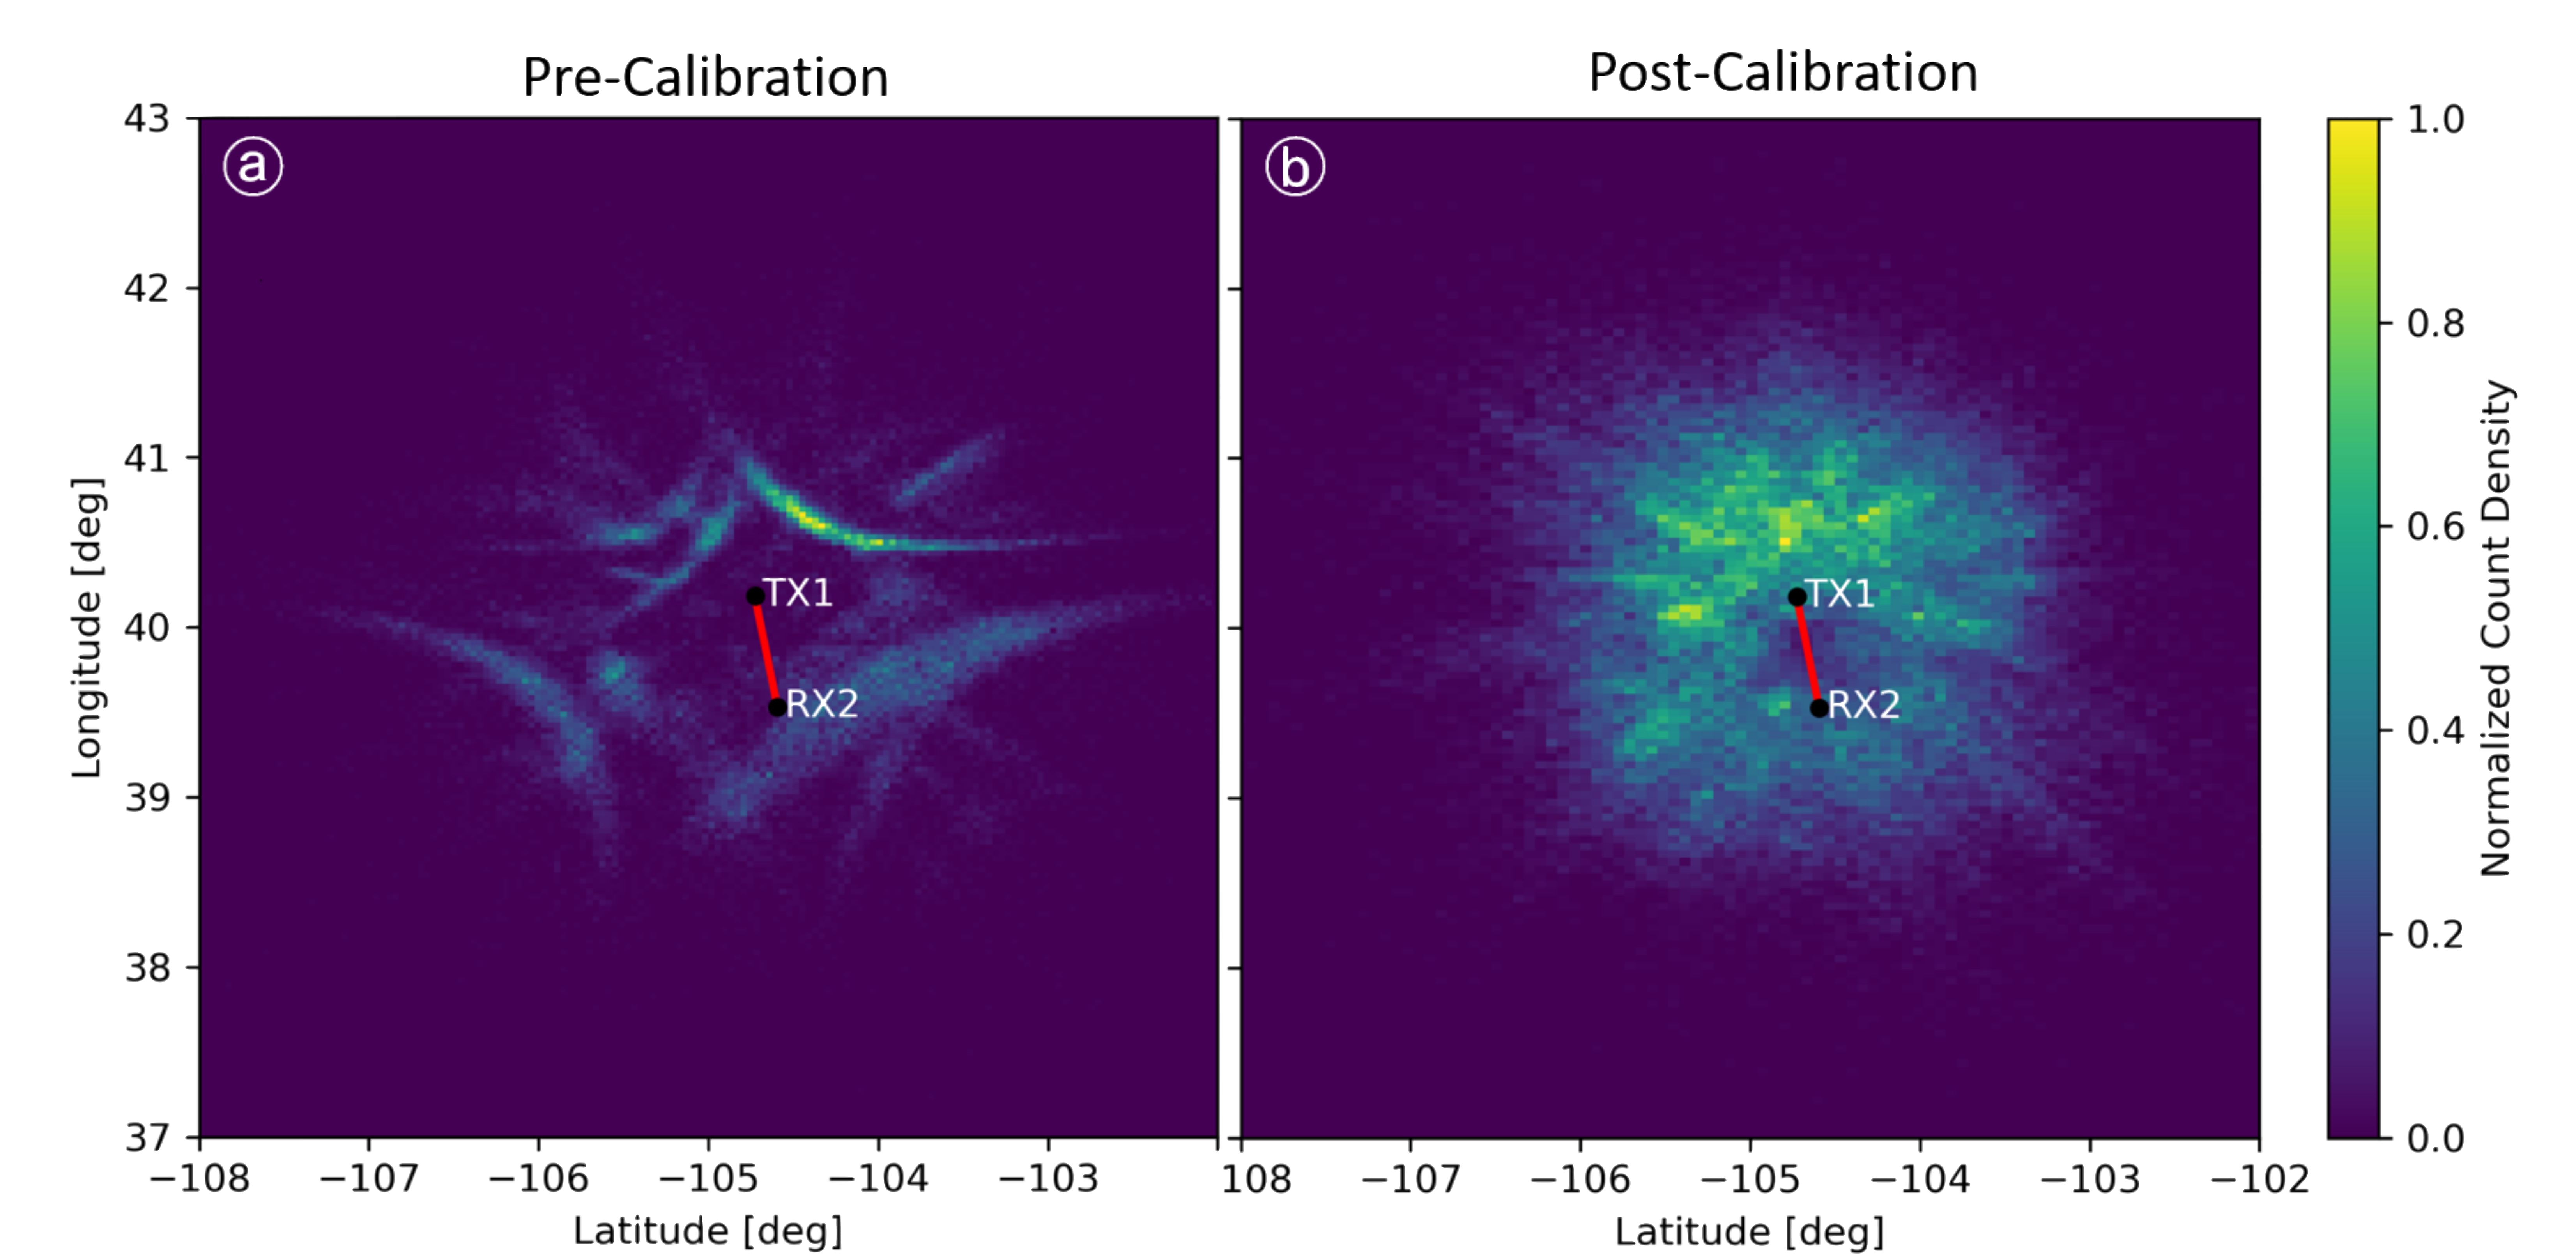
\includegraphics[width=0.85\linewidth]{img/calibration2.png}
                };
                \node[anchor=south, inner sep=2pt] at ([yshift=0.25cm, xshift=0.6cm]img.south) { 
                    {{{\fontsize{3}{3.4}\selectfont\raggedleft \textcolor{white}{\textit{Credit:} \citeauthor{marino_MeteorRadarPhase_2024}, \citeyear{marino_MeteorRadarPhase_2024} \cite{marino_MeteorRadarPhase_2024}}}}}
                };
            \end{tikzpicture}
            % 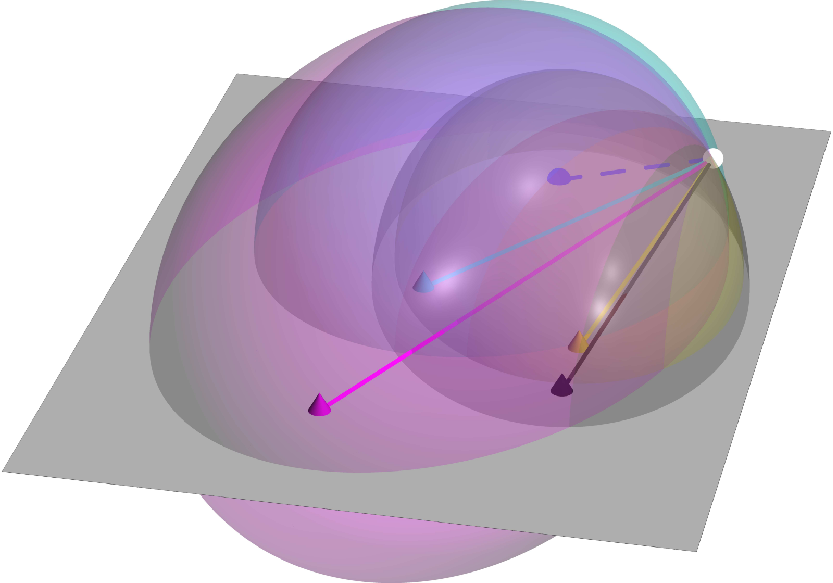
\includegraphics[width=0.65\linewidth]{img/4ellipsoids_compressed.pdf}
            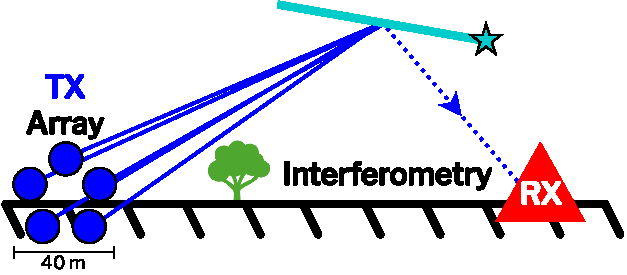
\includegraphics[width=\linewidth]{img/IF_basis_labeled.pdf}
            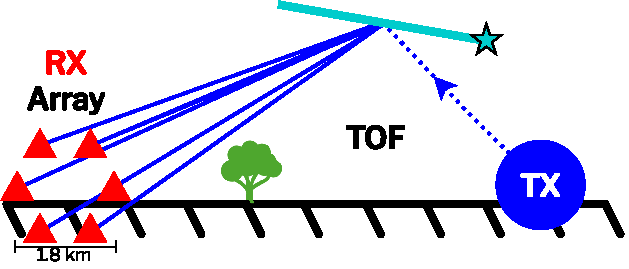
\includegraphics[width=\linewidth]{img/TOF_basis_labeled.pdf}
        \end{column}
    \end{columns}
\end{frame}